\section{Results}\label{sec:Results}

\subsection{Mortgage Classifier (Benchmark)}\label{subsec:Mortgage Classifier (Benchmark) Results}

In order to assess whether a predictive algorithm would pick up on and reproduce bias in the data, an initial classification model (as described in \textbf{chapter \ref{subsec:Model_Training_and_Prediction}} and detailed in \textbf{table \ref{tab:CH03_Model_Details}}) was trained on the HMDA dataset (see \textbf{chapter \ref{subsec:HMDA_Data}}) with the goal of predicting whether a mortgage would be granted or not for a given applicant.
The results of this model were assessed in terms of performance and fairness.

\textbf{Performance Assessment}

When fitting the neural network to the training data, the \textit{training accuracy} of the model improved rapidly initially, leveling off after a few epochs. The \textit{validation accuracy} started at a high level and constantly improved by small increments, suggesting that both the model learning process as well as the ability to generalize to previously unseen data were successful. 
% The training process was stopped by an early\_stopping callback, with the ninth epoch being the one with the least validation loss. The training results of the best epoch were:
The training process was stopped by an early\_stopping callback. The training results of the best epoch were:
\begin{itemize}
    \item \textit{Training Accuracy}: 0.90
    \item \textit{Validation Accuracy}: 0.90
    \item \textit{Training Loss}: 0.28
    \item \textit{Validation Loss}: 0.28
\end{itemize}
The history of the training process is depicted in subplot a) of \textbf{figure \ref{fig:Model_Training_Results_Panel}}.

%\begin{figure}
%    \centering
%    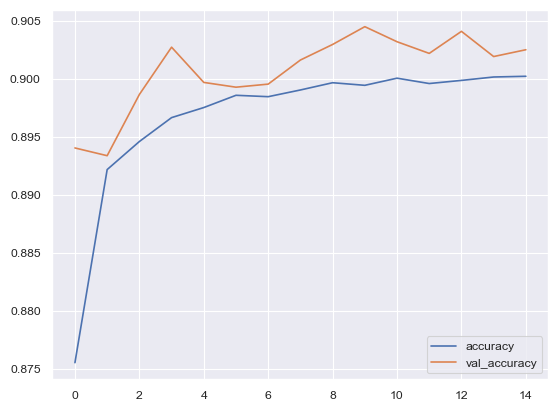
\includegraphics[width=0.85\textwidth]{images/Model_Training/Initial_Training_History.png}
%    \caption{Training History of the Mortgage Classifier Model}
%    \medskip
%    \small
%    The training history of the initial mortgage classifier model, showing the training and validation accuracy and loss over the course of the training process. The training accuracy improved constantly until the early\_stopping callback. The validation accuracy constantly improved, suggesting a successful learning process.
%    \label{fig:Model_Training_History}
%\end{figure}

The model was then evaluated on the test dataset, which was not seen by the model during training. The results of the performance evaluation (i.e. \textit{metrics \#1}) are shown in \textbf{table \ref{tab:Model_Evaluation}}. The model achieved an \textit{accuracy} of 0.90, a \textit{precision} of 0.88, a \textit{recall} of 0.97, and an \textit{F1-score} of 0.92. 
As stated in \textbf{chapter \ref{subsec:Model_Training_and_Prediction}}, the original model output were probabilities between 0 and 1. These could be used to calculate ROC AUC and plot the corresponding ROC curve, which can be seen in subplot b) of \textbf{figure \ref{fig:Model_Training_Results_Panel}}. The \textit{ROC-AUC} score was 0.94, indicating a high level of model performance. 
Converting the probabilities into predictions with a threshold of 0.5 fulfilled the classification requirement. The \textit{confusion matrix} is depicted in subplot c) of \textbf{figure \ref{fig:Model_Training_Results_Panel}}. The model managed to achieve a high number of true positives and true negatives, while the number of false negatives was low. However, the number of false positives was nearly 8\% of all predictions.

\begin{table}[!htbp]
    \centering
    \begin{tabular}{l c}
    \toprule
    \textbf{Metric} & \textbf{Value} \\
    \midrule
    \textbf{accuracy} & 0.90 \\
    \textbf{precision} & 0.88 \\
    \textbf{recall} & 0.97 \\
    \textbf{f1} & 0.92 \\
    \bottomrule
    \end{tabular}
%    \caption{Metrics \#1: Initial Model}
%    \small
%    The mortgage classifier model was evaluated on the test dataset, achieving an accuracy of 0.90, a precision of 0.88, a recall of 0.97, and an F1-score of 0.92.
    \medskip
    \caption[Metrics \#1: Initial Model]{\textbf{Metrics \#1: Initial Model} - The mortgage classifier model was evaluated on the test dataset, achieving an accuracy of 0.90, a precision of 0.88, a recall of 0.97, and an F1-score of 0.92.}
    \label{tab:Model_Evaluation}
\end{table}

%\begin{figure}
%    \centering
%    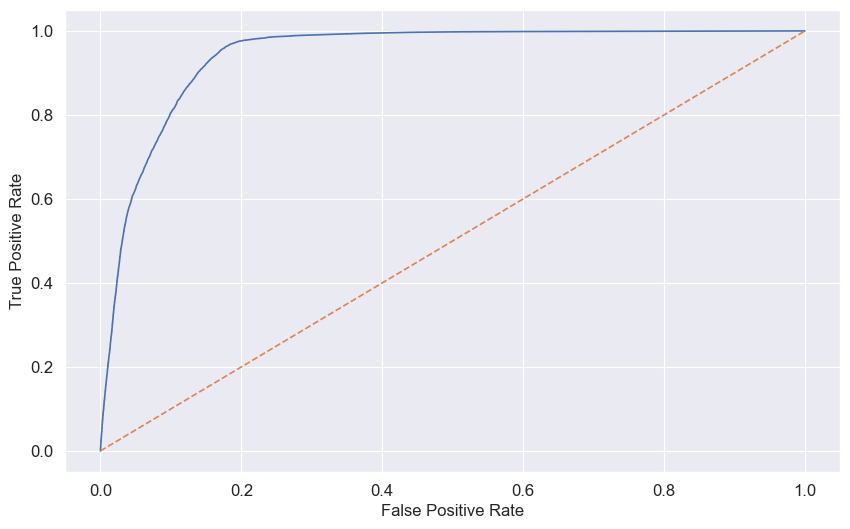
\includegraphics[width=0.85\textwidth]{images/Model_Training/Initial_ROC_curve.png}
%    \caption{ROC curve of the Mortgage Classifier Model}
%    \medskip
%    \small
%    The ROC curve is significantly above the diagonal baseline, indicating high predictive performance.
%    \label{fig:Model_Training_ROC}
%\end{figure}

%\begin{figure}
%    \centering
%    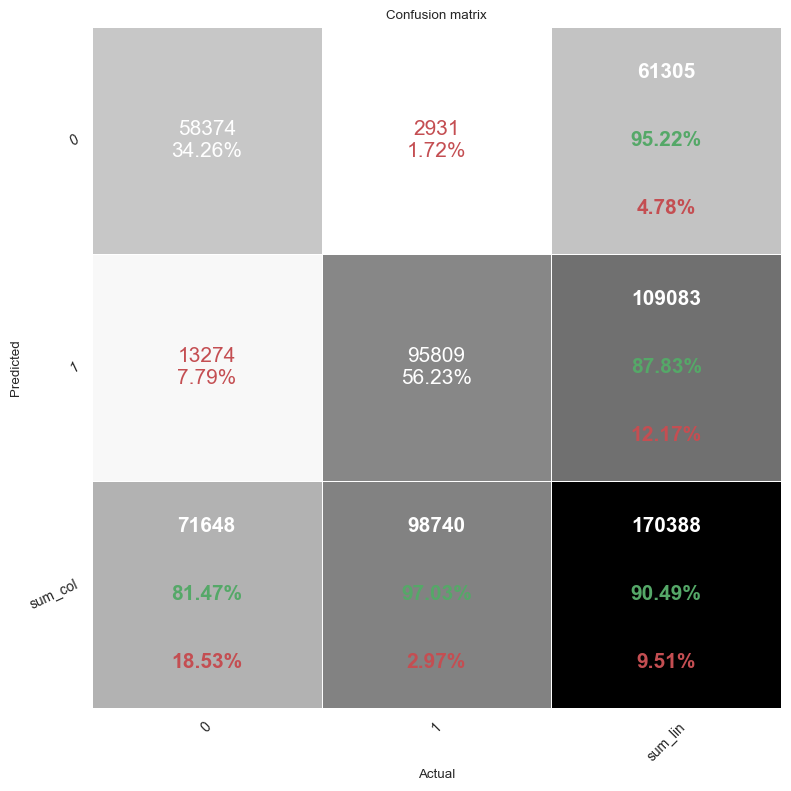
\includegraphics[width=0.85\textwidth]{images/Model_Training/Initial_Confusion_Matrix.png}
%    \caption{Confusion Matrix on the Test Dataset of the Mortgage Classifier Model}
%    \medskip
%    \small
%    The confusion matrix of the mortgage classifier model on the test dataset. The model achieved a high number of true positives and true negatives. The number of false negatives was low, however, false positives made up nearly 8\% of all predictions.
%    \label{fig:Model_Confusion_Matrix}
%\end{figure}

\begin{figure}[!htbp]

    \begin{center}

    \begin{minipage}[b]{0.5\textwidth}
        \centering
        \begin{subfigure}[t]{0.06\textwidth}
            \textbf{a)}
        \end{subfigure}
        \begin{subfigure}[t]{0.9\textwidth}
            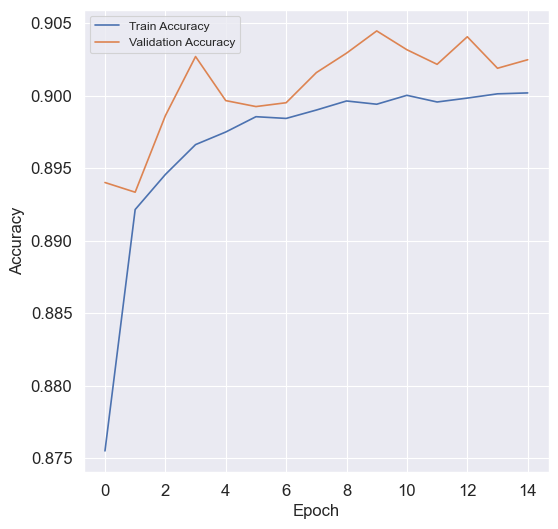
\includegraphics[width=\linewidth, valign=t]{images/Model_Training/Initial_Training_History_square.png}
        \end{subfigure}
    \end{minipage}%
    \begin{minipage}[b]{0.5\textwidth}
        \centering
        \begin{subfigure}[t]{0.06\textwidth}
            \textbf{b)}
        \end{subfigure}
        \begin{subfigure}[t]{0.9\textwidth}
            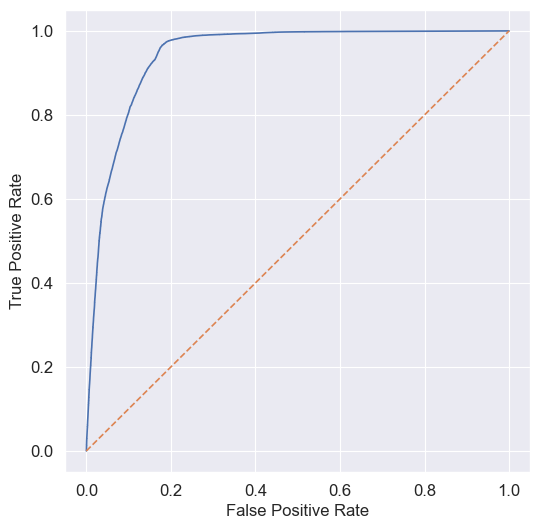
\includegraphics[width=\linewidth, valign=t]{images/Model_Training/Initial_ROC_curve_square.png}
        \end{subfigure}
    \end{minipage}%
    \hfill\allowbreak%
    \begin{minipage}[b]{0.75\textwidth}
        \centering
        \begin{subfigure}[t]{0.06\textwidth}
            \textbf{c)}
        \end{subfigure}
        \begin{subfigure}[t]{0.9\textwidth}
            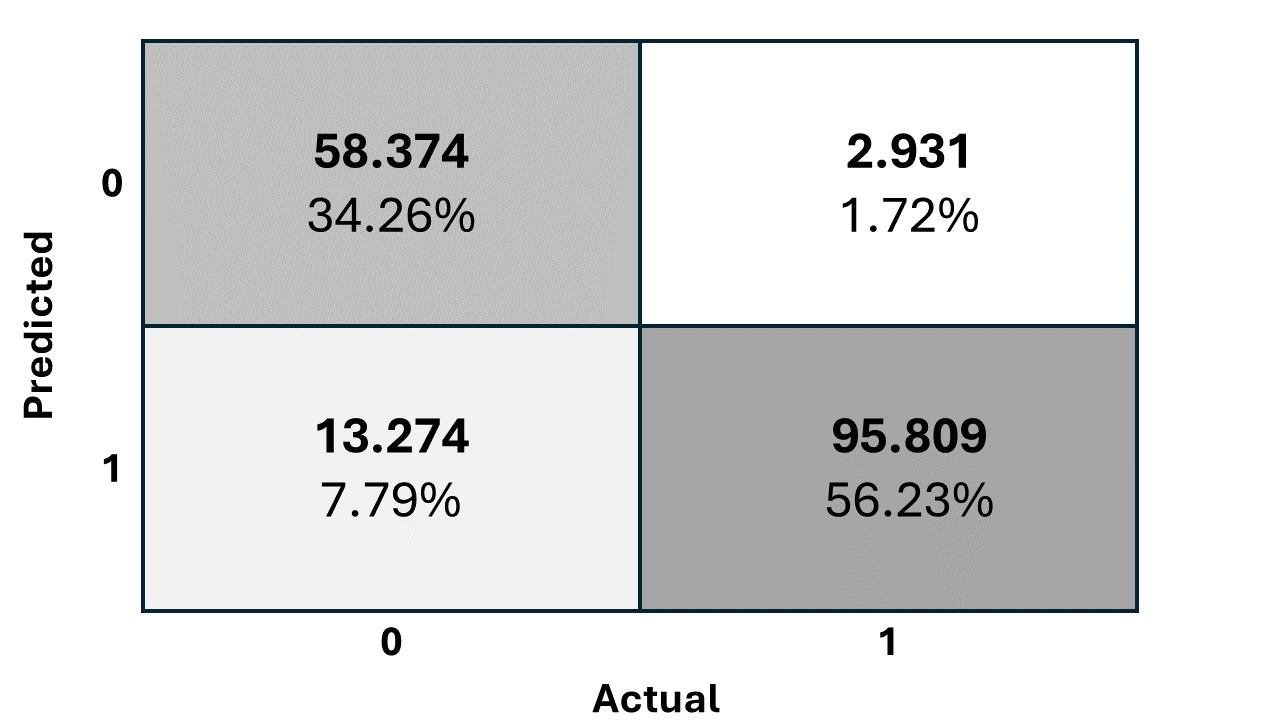
\includegraphics[width=\linewidth, valign=t]{images/Model_Training/Initial_Confusion_Matrix_PP.png}
        \end{subfigure}
    \end{minipage}
    \end{center}

    \caption[Training History, ROC curve, and Confusion Matrix of the Mortgage Classifier Model]{\textbf{Training History, ROC curve, and Confusion Matrix of the Mortgage Classifier Model} - \textbf{a)} The training history of the initial mortgage classifier model, showing the training and validation accuracy and loss over the course of the training process. 
    The training accuracy improved constantly until the early\_stopping callback. The validation accuracy constantly improved, suggesting a successful learning process.
    \textbf{b)} The ROC curve is significantly above the diagonal baseline, indicating high predictive performance. 
    \textbf{c)} The confusion matrix of the mortgage classifier model on the test dataset. The model achieved a high number of true positives and true negatives. The number of false negatives was low, however, false positives made up nearly 8\% of all predictions.}

    \label{fig:Model_Training_Results_Panel}

\end{figure}

\pagebreak

\textbf{Fairness Assessment}

Following the research question (see \textbf{chapter \ref{ch:Introduction}}), the \textit{detection of unfairness} in the predictions is an explicit goal of this thesis. To address this, the fairness assessment outlined in \textbf{chapter \ref{subsec:Model_Training_and_Prediction}} was applied to the predictions. The results of the fairness assessment (i.e. \textit{metrics \#2}) are shown in \textbf{table \ref{tab:Fairness_Assessment_Initial}}. 
The model performed slightly better for \textit{White} applicants than for \textit{Black} applicants. The \textit{accuracy} for \textit{White} applicants was 0.91, while it was 0.88 for \textit{Black} applicants. The \textit{precision} for \textit{White} applicants was 0.89, while it was 0.82 for \textit{Black} applicants. The \textit{recall} for \textit{White} applicants was 0.97, while it was 0.96 for \textit{Black} applicants. 
The \textit{F1-score} for \textit{White} applicants was 0.93, while it was 0.88 for \textit{Black} applicants. The \textit{AUC} for \textit{White} applicants was 0.94, while it was 0.95 for \textit{Black} applicants. 
In terms of disparities (where the optimal value is \textbf{1}), the model performed comparably well in all disciplines except the \textit{fnr\_disparity}, which was 1.42. This indicates that the model was more likely to predict a false negative for \textit{Black} applicants than for \textit{White} applicants.

\begin{table}[!htbp]
    \centering
    \begin{tabular}{lr}
    \toprule
    \textbf{Metric} & \textbf{Value} \\
    \midrule
    \textbf{Accuracy White} & 0.91 \\
    \textbf{Precision White} & 0.89 \\
    \textbf{Recall White} & 0.97 \\
    \textbf{F1 Score White} & 0.93 \\
    \textbf{AUC White} & 0.94 \\
    \midrule
    \textbf{Accuracy Black} & 0.88 \\
    \textbf{Precision Black} & 0.82 \\
    \textbf{Recall Black} & 0.96 \\
    \textbf{F1 Score Black} & 0.88 \\
    \textbf{AUC Black} & 0.95 \\
    \midrule
    \textbf{tpr\_disparity} & 0.99 \\
    \textbf{fpr\_disparity} & 0.96 \\
    \textbf{tnr\_disparity} & 1.01 \\
    \textbf{fnr\_disparity} & 1.42 \\
    \bottomrule
    \end{tabular}
%    \caption{Metrics \#2: Initial Model}
    \medskip
    \caption[Metrics \#2: Initial Model]{\textbf{Metrics \#2: Initial Model} - The benchmark model showed a slightly better performance for \textit{White} applicants than for \textit{Black} applicants. The disparities were comparably low, except for the \textit{fnr\_disparity}, which was 1.42.}
    \label{tab:Fairness_Assessment_Initial}
%    \small
%    The benchmark model showed a slightly better performance for \textit{White} applicants than for \textit{Black} applicants. The disparities were comparably low, except for the \textit{fnr\_disparity}, which was 1.42.
\end{table}

\subsection{Explainability}\label{Explainability Results}

As stated in \textbf{chapter \ref{subsec:Explainability}}, three different approaches to explainability were utilized not only to support the analysis of fairness by providing insights into the model's decision-making process, but also to provide a better understanding of the model's behavior: \textit{SHAP}, \textit{LIME}, and a \textit{Global Surrogate Model}. 

\textbf{SHAP}

As stated in \textbf{chapter \ref{subsec:algorithms}}, the SHAP algorithm tries to game-theoretically distribute the value of the final prediction among the individual features considered.
\textbf{Figure \ref{fig:SHAP_beeswarm}} shows the SHAP beeswarm plot, which displays the distribution of the SHAP values for each feature in the dataset. The color indicates the feature value (red = higher; blue = lower), while the x-axis shows the SHAP value (left of center = negative; right of center = positive). The y-axis shows the feature name. The plot includes 150 values from the SHAP values of the test dataset.
It showed that the most influential features according to SHAP were \textit{debt\_to\_income\_ratio\_missing, interest\_rate, loan\_to\_value\_ratio}, and \textit{debt\_to\_income\_ratio\_>60\%}.
While it was apparent how missingness in the debt to income ratio (missingness is negative, availability is positive) and values >60\% in the debt to income ratio (higher is negative, lower is positive) affected the model decision, interest rates and the loan-to-value-ratios as the numerical variables were less intuitive to interpret.
Although most medium to high interest rates seemed to be related with slight negative impacts, there also was a cluster of higher values for these variables corresponding with positive prediction influences.
As all other variables were categorical, their interpretations were straightforward. Albeit their absolute impact in terms of SHAP values was limited, it is noteworthy that the \textit{protected variables} of race and sex were in fact picked up on by the model.
In every case where a decision was negatively influenced by the \textit{race} of the applicant, the applicant in question was Black or African American (as can be inferred from all values left of the center of the x-axis for \textit{applicant\_race-1\_White} being colored blue for this feature, meaning a lower value, which in turn means Black or African American ethnicity).
A similar picture was observed for the \textit{sex} of the applicant: In most cases where the model picked up on the sex being an influential factor on the model decision, the applicant in question was \textit{female} and vice versa.

\begin{figure}[!htbp]
    \centering
    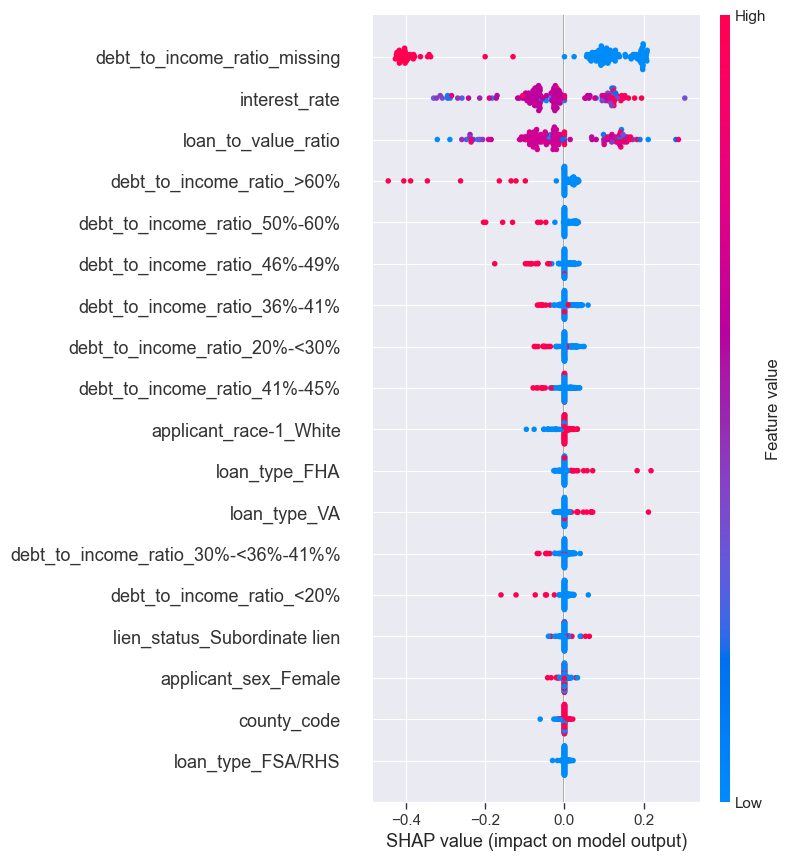
\includegraphics[width=0.85\textwidth]{images/SHAP_Individual_Analyses/beeswarm.png}
%    \caption{SHAP beeswarm plot}
%    \medskip
%    \small
%    The SHAP beeswarm plot shows the distribution of the SHAP values for each feature in the dataset. The color indicates the feature value, while the x-axis shows the SHAP value. The y-axis shows the feature name.
    \caption[SHAP beeswarm plot]{\textbf{SHAP beeswarm plot} - The SHAP beeswarm plot shows the distribution of the SHAP values for each feature in the dataset. The color indicates the feature value, while the x-axis shows the SHAP value. The y-axis shows the feature name.}
    \label{fig:SHAP_beeswarm}
\end{figure}

The \textit{expected value} of the SHAP values (i.e. the baseline before consideration of any feature importance) was \textit{0.57}. This corresponds to the imbalance in the original HMDA data (see \textbf{chapter \ref{fig:CHXX_Target_Variable_Distribution}}).
\textbf{Figure \ref{fig:SHAP_Individual_Analyses}} shows the SHAP values for four selected applicants. The force plots displayed show how the individual values of the features influence the model's decision according to SHAP. 
Each individual prediction results from the aforementioned \textit{expected value} and the sum of inferred importances of the features (exemplarily, in the first plot displayed in \textbf{figure \ref{fig:SHAP_Individual_Analyses}}, the feature importances amount to roughly positive 0.4, leading to a total value of 0.97 and therefore a positive prediction, i.e. a granted mortgage).
It shows that SHAP attributes a high importance to (missingness of) the Debt to income ratio. Due to the values being scaled, a value of \textit{-0.59} corresponds to \textit{debt\_to\_income\_ratio\_missing == False} and a value of \textit{1.68} corresponds to \textit{debt\_to\_income\_ratio\_missing == True}. Therefore, SHAP considers missingness in this variable as negative and availability as positive.
Considering the last applicant displayed (\textit{Black or African American Male, Debt to Income Ratio available}), it does however show that even availabilty of the Debt to Income Ratio does not guarantee a positive model decision.
According to SHAP, none of the decisions displayed here (and in the whole set of predictions in general) were significantly informed by any protected attribute. However, confounding factors might still be present, as the model might have learned to discriminate based on other features that are correlated with the protected attributes.

\begin{figure}[!htbp]
    \centering
    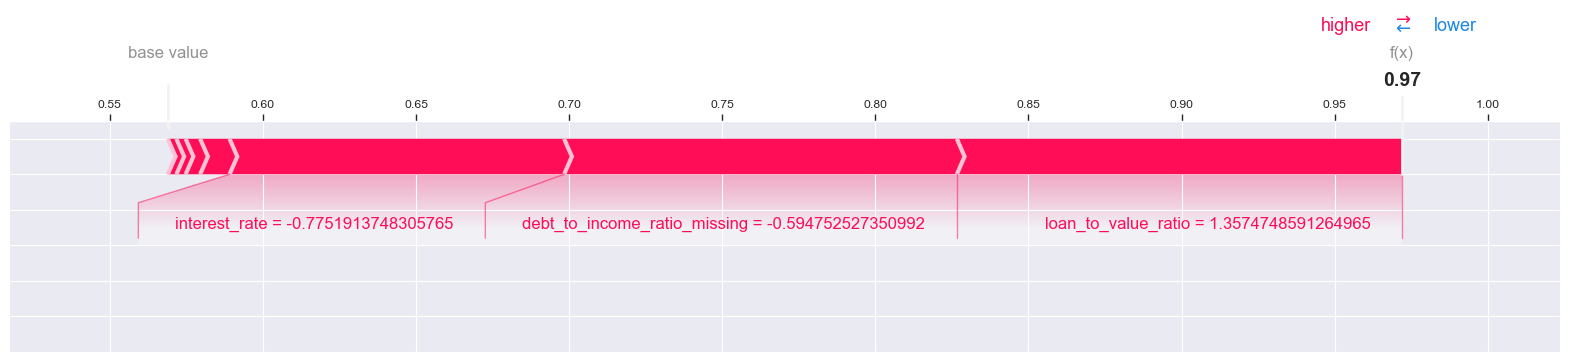
\includegraphics[width=0.95\textwidth]{images/SHAP_Individual_Analyses/SHAP_individual_0.png}
    \small
    White Male, Debt to Income Ratio available
    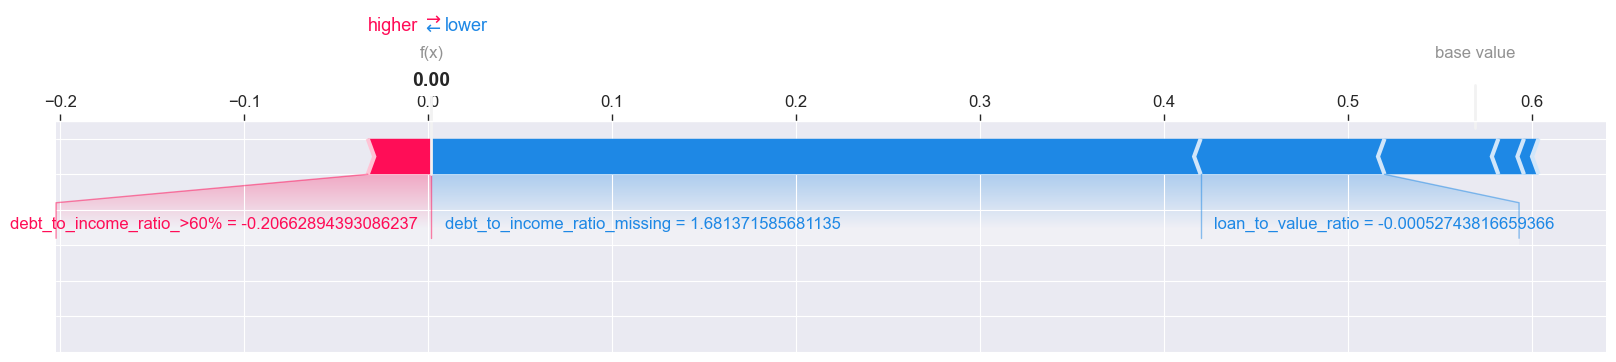
\includegraphics[width=0.95\textwidth]{images/SHAP_Individual_Analyses/SHAP_individual_1.png}
    \small
    White Male, Debt to Income Ratio missing
    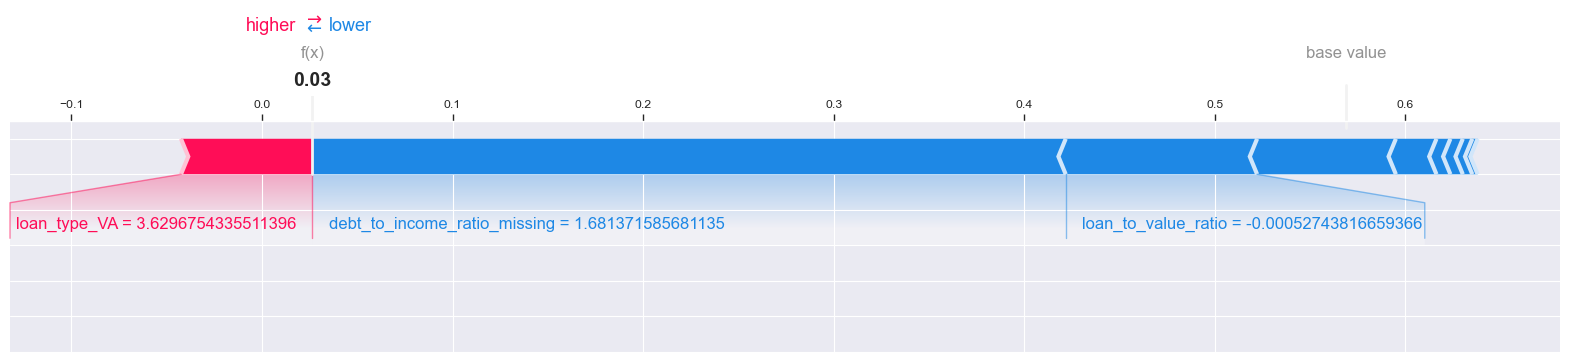
\includegraphics[width=0.95\textwidth]{images/SHAP_Individual_Analyses/SHAP_individual_21.png}
    \small
    Black or African American Male, Debt to Income Ratio missing
    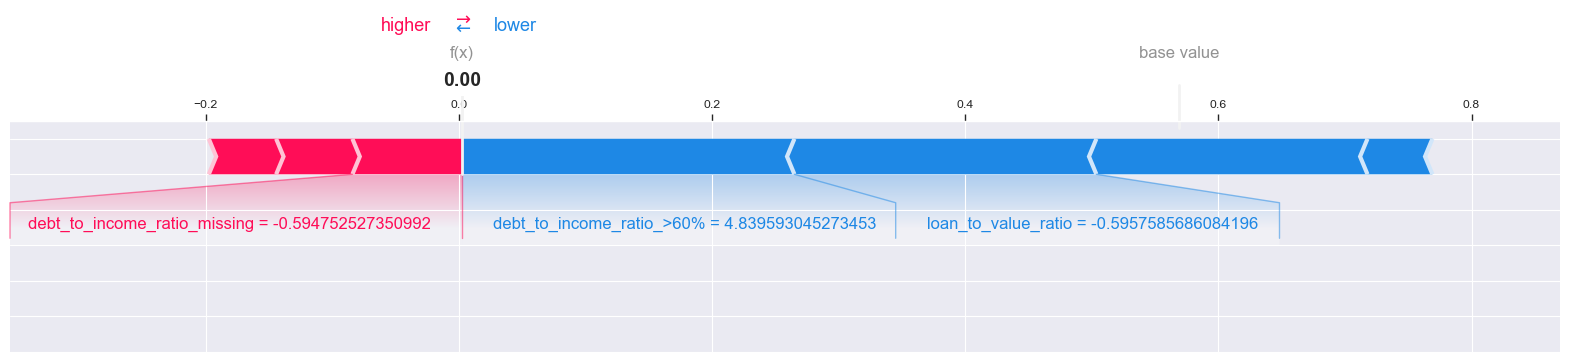
\includegraphics[width=0.95\textwidth]{images/SHAP_Individual_Analyses/SHAP_individual_139.png}
    \small
    Black or African American Male, Debt to Income Ratio available
%    \caption{Selected SHAP Individual Analyses}
%    \medskip
%    \small
%    Comparing four selected Male applicants with different characteristics shows that, in general, SHAP attributes a high importance to (missingness of) the Debt to Income Ratio. However, it is not the sole decision criterion, as the last applicant displayed shows.
    \medskip
    \caption[Selected SHAP Individual Analyses]{\textbf{Selected SHAP Individual Analyses} - Comparing four selected Male applicants with different characteristics shows that, in general, SHAP attributes a high importance to (missingness of) the Debt to Income Ratio. However, it is not the sole decision criterion, as the last applicant displayed shows.}
    \label{fig:SHAP_Individual_Analyses}
\end{figure}

\pagebreak

\textbf{LIME}

The LIME algorithm, in contrast to SHAP, tries to explain the model's decision on a local level by approximating the model's behavior around a single prediction (see \textbf{chapter \ref{subsec:algorithms}}).
\textbf{Figure \ref{fig:LIME_Individual_Analyses}} shows the LIME individual feature importance plot for a selected applicant, specifically the same applicant that is denoted as \textit{White Male, Debt to Income Ratio available} in \textbf{figure \ref{fig:SHAP_Individual_Analyses}}. The x-axis shows the feature importance, while the y-axis shows the feature name.
It showed that LIME attributes a high importance to the \textit{loan type} and the \textit{debt to income ratio}. Once again, the \textit{protected attributes} had very little absolute influence on the model's decision according to LIME.

\begin{figure}[!htbp]
    \centering
    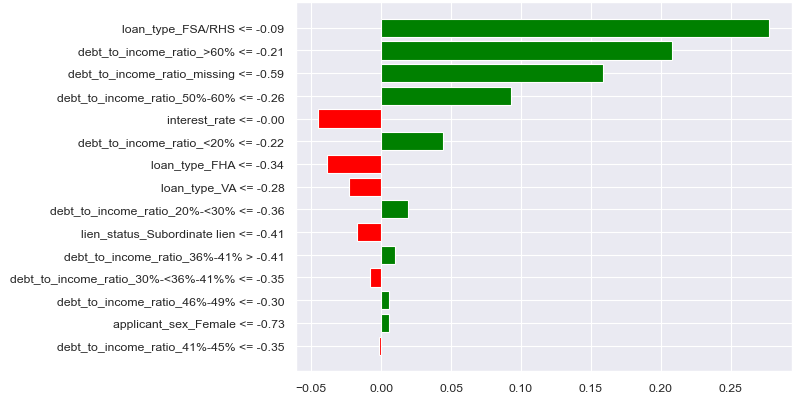
\includegraphics[width=0.95\textwidth]{images/CHXX_LIME_individual.png}
%    \caption{LIME Individual Feature Importance}
%    \medskip
%    \small
%    The LIME individual feature importance plot shows the direction and the impact of the features on the model's decision for a selected applicant. The x-axis shows the feature importance, while the y-axis shows the feature name.
    \caption[LIME Individual Feature Importance]{\textbf{LIME Individual Feature Importance} - The LIME individual feature importance plot shows the direction and the impact of the features on the model's decision for a selected applicant. The x-axis shows the feature importance, while the y-axis shows the feature name.}
    \label{fig:LIME_Individual_Analyses}
\end{figure}

While the overall explanations on which features are influential are similar for both SHAP and LIME, the actual impact of the features varies significantly. While this is not a direct threat to the quality of the results of this thesis, it is a reminder that explainability algorithms need to be analyzed carefully. 
This ties with the findings of Krishna et al. \parencite{Krishna2022}, who emphasize the importance of understanding the underlying assumptions of explainability algorithms and the need for a more comprehensive evaluation of their results.

\textbf{Global Surrogate Model}

To validate the results of the local explanations, a \textit{Global Surrogate Model} was used. \textbf{figure \ref{fig:Global_Surrogate}} shows the results of the global surrogate model. Specifically, the five most important features according to the global surrogate model are compared to the SHAP and LIME explanations in terms of their relative performance.
It showed that all three explanation algorithms mainly agree on the three most important features in the data (\textit{debt\_to\_income\_ratio\_missing, interest\_rate}, and \textit{debt\_to\_income\_ratio\_>60\%}), although LIME attributes a different order of importance to them compared to SHAP and the global surrogate model.

\begin{figure}[!htbp]
    \centering
    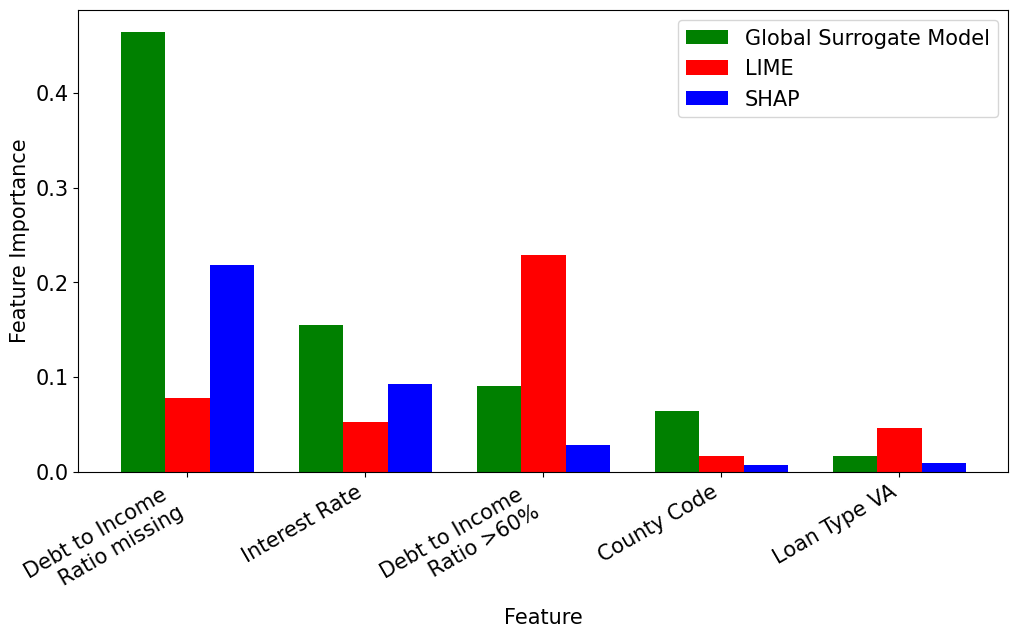
\includegraphics[width=0.85\textwidth]{images/CHXX_UPDATE_Surrogate_SHAP_LIME_combined.png}
%    \caption{Global Surrogate Model compared to SHAP and LIME}
%    \medskip
%    \small
%    Analyzing the 5 most important features according to the global surrogate model implies that the overall trends of SHAP and LIME are close to the global explanations.
    \caption[Global Surrogate Model compared to SHAP and LIME]{\textbf{Global Surrogate Model compared to SHAP and LIME} - Analyzing the 5 most important features according to the global surrogate model implies that the overall trends of SHAP and LIME are close to the global explanations. Although LIME attributes a higher importance to the \textit{Debt to Income Ratio} being >60\%, than to missingness, the three most important features are similar in all three models.}
    \label{fig:Global_Surrogate}
\end{figure}

\textbf{Summary}

While the SHAP and LIME algorithms agreed on the most important features, the actual impact of these features varied significantly. The global surrogate model confirmed the results of the local explanations, showing that the most important features were the \textit{debt to income ratio} and the \textit{interest rate}. 
It is noteworthy that missingness in the \textit{debt\_to\_income\_ratio} cannot be considered to be at random as it is highly predictive of the model's decision. 
While individual values put out by SHAP and LIME might differ due to the different approaches, the overall trends of the explanations were similar, suggesting that the model's decision-making process could be explained with some level of confidence.

\pagebreak

\subsection{Fairness Adjustments}\label{Fairness Adjustments Results}

While the performance of the benchmark mortgage classifier detailed in \textbf{chapter \ref{subsec:Mortgage Classifier (Benchmark) Results}} was satisfactory, the scope of this thesis (see \textbf{chapter \ref{ch:Introduction}}) included taking an iterative approach to improve fairness without sacrificing predictive performance, as outlined in \textbf{chapter \ref{subsec:Iterations}}.
To this end, the following fairness adjustments were applied to the model: \textit{Reweighing}, \textit{Correlation Remover} and \textit{Calibrated Equalized Odds}. The aim was to reach improvement in at least one of the two metric sets, compared to the benchmark performance depicted in \textbf{table \ref{tab:Model_Evaluation}} (\textit{metrics \#1}) and \textbf{table \ref{tab:Fairness_Assessment_Initial}} (\textit{metrics \#2}).

\textbf{Reweighing}

Using the \textit{reweighing} pre-processing algorithm to assign specific weights to the training data without actually adjusting the underlying data (for details, refer to \textbf{chapter \ref{subsec:Iterations}}), yielded positive results in terms of model performance.
While the predictive performance of the model (as measured by \textit{metrics \#1}) could be kept on the same level that was reached by the benchmark model (see \textbf{table \ref{tab:Model_Evaluation_Reweighing}}), the fairness in terms of the disparities in predictions between \textit{White} and \textit{Black or African American} applicants could be reduced in comparison (see \textbf{table \ref{tab:Fairness_Assessment_Reweighing}})

\begin{table}[!htbp]
    \centering
    \begin{tabular}{l c}
    \toprule
    \textbf{Metric} & \textbf{Value} \\
    \midrule
    \textbf{accuracy} & 0.90 \\
    \textbf{precision} & 0.88 \\
    \textbf{recall} & 0.97 \\
    \textbf{f1} & 0.92 \\
    \bottomrule
    \end{tabular}
%    \caption{Metrics \#1: Reweighing}
%    \small
%    The performance of the \textit{reweighed} model was on par with the benchmark (compare \textbf{table \ref{tab:Model_Evaluation}}).
    \medskip
    \caption[Metrics \#1: Reweighing]{\textbf{Metrics \#1: Reweighing} - The performance of the \textit{reweighed} model was on par with the benchmark (compare \textbf{table \ref{tab:Model_Evaluation}}).}
    \label{tab:Model_Evaluation_Reweighing}
\end{table}

\begin{table}[h]%[!htbp]
    \centering
    \begin{tabular}{lr}
    \toprule
    \textbf{Metric} & \textbf{Value} \\
    \midrule
    \textbf{Accuracy White} & 0.91 \\
    \textbf{Precision White} & 0.89 \\
    \textbf{Recall White} & 0.97 \\
    \textbf{F1 Score White} & 0.93 \\
    \textbf{AUC White} & 0.94 \\
    \midrule
    \textbf{Accuracy Black} & 0.88 \\
    \textbf{Precision Black} & 0.81 \\
    \textbf{Recall Black} & 0.97 \\
    \textbf{F1 Score Black} & 0.88 \\
    \textbf{AUC Black} & 0.95 \\
    \midrule
    \textbf{tpr\_disparity} & 0.99 \\
    \textbf{fpr\_disparity} & 1.00 \\
    \textbf{tnr\_disparity} & 1.00 \\
    \textbf{fnr\_disparity} & 1.20 \\
    \bottomrule
    \end{tabular}
%    \caption{Metrics \#2: Reweighing}
    \medskip
    \caption[Metrics \#2: Reweighing]{\textbf{Metrics \#2: Reweighing} - While the subgroup performances of the \textit{reweighed} model were comparable to those of the benchmark model (compare \textbf{table \ref{tab:Fairness_Assessment_Initial}}), the disparities were nearly nullified with the exception of the \textit{fnr disparity}, which still is on a good level with 1.20.}
    \label{tab:Fairness_Assessment_Reweighing}
%    \small
%    While the subgroup performances of the \textit{reweighed} model were comparable to those of the benchmark model (compare \textbf{table \ref{tab:Fairness_Assessment_Initial}}), the disparities were nearly nullified with the exception of the \textit{fnr disparity}, which still is on a satisfactory level with 1.20.
\end{table}

\textbf{Correlation Remover}

As described in \textbf{chapter \ref{subsec:Iterations}}, the \textit{correlation remover} algorithm aims to minimize any correlation of selected protected attributes with any other variables within the data.
While the performance of the model (see \textbf{table \ref{tab:Model_Evaluation_Corr_Rem}}) with the accordingly data pre-processed was comparable to or in parts slightly better than the benchmark model (compare \textbf{table \ref{tab:Model_Evaluation}}), it did not perform well in terms of fairness (see \textbf{table \ref{tab:Fairness_Assessment_Corr_Rem}}).
Subgroup performance could not be optimized compared to the benchmark and the disparities were higher, indicating less equality in the model predictions.

\begin{table}[!htbp]
    \centering
    \begin{tabular}{l c}
    \toprule
    \textbf{Metric} & \textbf{Value} \\
    \midrule
    \textbf{accuracy} & 0.91 \\
    \textbf{precision} & 0.88 \\
    \textbf{recall} & 0.97 \\
    \textbf{f1} & 0.92 \\
    \bottomrule
    \end{tabular}
%    \caption{Metrics \#1: Correlation Remover}
%    \small
%    The performance of the \textit{correlation remover} model was very similar to the benchmark (compare \textbf{table \ref{tab:Model_Evaluation}}).
    \medskip
    \caption[Metrics \#1: Correlation Remover]{\textbf{Metrics \#1: Correlation Remover} - The performance of the \textit{correlation remover} model was very similar to the benchmark (compare \textbf{table \ref{tab:Model_Evaluation}}).}
    \label{tab:Model_Evaluation_Corr_Rem}
\end{table}

\begin{table}[h]%[!htbp]
    \centering
    \begin{tabular}{lr}
    \toprule
    \textbf{Metric} & \textbf{Value} \\
    \midrule
    \textbf{Accuracy White} & 0.91 \\
    \textbf{Precision White} & 0.89 \\
    \textbf{Recall White} & 0.97 \\
    \textbf{F1 Score White} & 0.93 \\
    \textbf{AUC White} & \text{NA} \\
    \midrule
    \textbf{Accuracy Black} & 0.89 \\
    \textbf{Precision Black} & 0.84 \\
    \textbf{Recall Black} & 0.93 \\
    \textbf{F1 Score Black} & 0.88 \\
    \textbf{AUC Black} & \text{NA} \\
    \midrule
    \textbf{tpr\_disparity} & 0.96 \\
    \textbf{fpr\_disparity} & 0.80 \\
    \textbf{tnr\_disparity} & 1.05 \\
    \textbf{fnr\_disparity} & 2.67 \\
    \bottomrule
    \end{tabular}
%    \caption{Metrics \#2: Correlation Remover}
    \medskip
    \caption[Metrics \#2: Correlation Remover]{\textbf{Metrics \#2: Correlation Remover} - While the subgroup performances of the \textit{correlation remover} model were comparable to those of the benchmark model (compare \textbf{table \ref{tab:Fairness_Assessment_Initial}}), the disparities had higher absolute distances from 1, indicating a lower level of fairness.}
    \label{tab:Fairness_Assessment_Corr_Rem}
%    \small
%    While the subgroup performances of the \textit{correlation remover} model were comparable to those of the benchmark model (compare \textbf{table \ref{tab:Fairness_Assessment_Initial}}), the disparities had higher absolute distances from 1, indicating a lower level of fairness.
\end{table}

\pagebreak

\textbf{Calibrated Equalized Odds}

The only postprocessing algorithm within the fairness adjustments, the \textit{calibrated equalized odds} algorithm (see \textbf{chapter \ref{subsec:Iterations}} for details), aims to adjust the model's predictions to ensure equalized odds between the protected attributes while keeping the results calibrated.
\textbf{Tables \ref{tab:Model_Evaluation_Cal_Eq_Odd}} and \textbf{\ref{tab:Fairness_Assessment_Cal_Eq_Odd}} show that the performance of this algorithm is not optimal within the context of this thesis. Both \textit{Metrics \#1} and \textit{Metrics \#2} indicate a lower performance of this algorithm compared to the benchmark (compare \textbf{table \ref{tab:Model_Evaluation}}).

\begin{table}[!htbp]
    \centering
    \begin{tabular}{l c}
    \toprule
    \textbf{Metric} & \textbf{Value} \\
    \midrule
    \textbf{accuracy} & 0.73 \\
    \textbf{precision} & 0.69 \\
    \textbf{recall} & 0.97 \\
    \textbf{f1} & 0.81 \\
    \bottomrule
    \end{tabular}
%    \caption{Metrics \#1: Calibrated Equalized Odds}
%    \small
%    Compared to the benchmark model (see \textbf{table \ref{tab:Fairness_Assessment_Initial}}), the model performance of the \textit{calibrated equalized odds} is significantly worse. Besides the \textit{recall}, which was kept on the same level, all performance metrics are well below those of the benchmark model.
    \medskip
    \caption[Metrics \#1: Calibrated Equalized Odds]{\textbf{Metrics \#1: Calibrated Equalized Odds} - Compared to the benchmark model (see \textbf{table \ref{tab:Fairness_Assessment_Initial}}), the model performance of the \textit{calibrated equalized odds} is significantly worse. Besides the \textit{recall}, which was kept on the same level, all performance metrics are well below those of the benchmark model.}
    \label{tab:Model_Evaluation_Cal_Eq_Odd}
\end{table}

\begin{table}[h]%[!htbp]
    \centering
    \begin{tabular}{lr}
    \toprule
    \textbf{Metric} & \textbf{Value} \\
    \midrule
    \textbf{Accuracy White} & 0.72 \\
    \textbf{Precision White} & 0.68 \\
    \textbf{Recall White} & 0.98 \\
    \textbf{F1 Score White} & 0.81 \\
    \textbf{AUC White} & \text{NA} \\
    \midrule
    \textbf{Accuracy Black} & 0.81 \\
    \textbf{Precision Black} & 0.73 \\
    \textbf{Recall Black} & 0.93 \\
    \textbf{F1 Score Black} & 0.82 \\
    \textbf{AUC Black} & \text{NA} \\
    \midrule
    \textbf{tpr\_disparity} & 0.95 \\
    \textbf{fpr\_disparity} & 0.43 \\
    \textbf{tnr\_disparity} & 2.23 \\
    \textbf{fnr\_disparity} & 3.25 \\
    \bottomrule
    \end{tabular}
%    \caption{Metrics \#2: Calibrated Equalized Odds}
    \medskip
    \caption[Metrics \#2: Calibrated Equalized Odds]{\textbf{Metrics \#2: Calibrated Equalized Odds} - Similar to the total performance of the model (see \textbf{table \ref{tab:Model_Evaluation_Cal_Eq_Odd}}), the performance of the \textit{calibrated equalized odds} model in terms of fairness was significantly worse than that of the benchmark model (see \textbf{table \ref{tab:Fairness_Assessment_Initial}}) for both subgroups, as were the disparities.}
    \label{tab:Fairness_Assessment_Cal_Eq_Odd}
%    \small
%    Similar to the total performance of the model (see \textbf{table \ref{tab:Model_Evaluation_Cal_Eq_Odd}}), the performance of the \textit{calibrated equalized odds} model in terms of fairness was significantly worse than that of the benchmark model (see \textbf{table \ref{tab:Fairness_Assessment_Initial}}) for both subgroups, as were the disparities.
\end{table}

\textbf{Summary}

Considering the overall \textit{performance} of the different approaches, all models except the \textit{calibrated equalized odds} algorithms performed on a similar, good level (see \textbf{table \ref{tab:metrics_1_iterations_summary}}).
The \textit{correlation removal} algorithm managed to slightly outperform the benchmark model in terms of \textit{accuracy}, \textit{precision}, and \textit{f1-score}, while the \textit{calibrated equalized odds} algorithm managed to slightly outperform the benchmark model in terms of \textit{recall}.

\begin{table}[!htbp]
    \centering
    \begin{tabular}{l *{4}{>{$}c<{$}}}
    \toprule
    & \textbf{Initial Model} & \textbf{Reweighing} & \textbf{Calibrated Equalized Odds} & \textbf{Correlation Removal} \\
    \midrule
    \textbf{accuracy} & 0.90 & 0.90 & 0.73 & \textbf{0.91} \\
    \textbf{precision} & 0.88 & 0.88 & 0.69 & \textbf{0.88} \\
    \textbf{recall} & 0.97 & 0.97 & \textbf{0.97} & 0.97 \\
    \textbf{f1} & 0.92 & 0.92 & 0.81 & \textbf{0.92} \\
    \textbf{roc\_auc} & \textbf{0.94} & 0.94 & \text{NA} & \text{NA} \\
    \bottomrule
    \end{tabular}
%    \caption{Metrics \#1: Fairness Adjustments Summary}
%    \small
%    Results of \textit{metrics \#1} for all applied algorithms. The values are rounded, the highest scores are marked \textbf{bold}.
    \medskip
    \caption[Metrics \#1: Fairness Adjustments Summary]{\textbf{Metrics \#1: Fairness Adjustments Summary} - Results of \textit{metrics \#1} for all applied algorithms. The values are rounded, the highest scores are marked \textbf{bold}.}
    \label{tab:metrics_1_iterations_summary}
\end{table}

In terms of \textit{fairness}, no significant optimizations could be achieved. The \textit{reweighing} technique managed to improve the overall fairness of the model, but the other techniques did not manage to reach the same level of fairness. 
\textbf{Figure \ref{fig:Bar_Grant_per_Race}} shows that the differences in loan grants between \textit{White} and \textit{Black or African American} applicants was not substantially reduced by any of the iterations, with the calibrated equalized odds algorithm even increasing the difference.

\begin{figure}[!htbp]

    \centering

    \begin{minipage}[b]{0.5\textwidth}
        \centering
        \begin{subfigure}[t]{0.06\textwidth}
            \textbf{a)}
        \end{subfigure}
        \begin{subfigure}[t]{0.9\textwidth}
            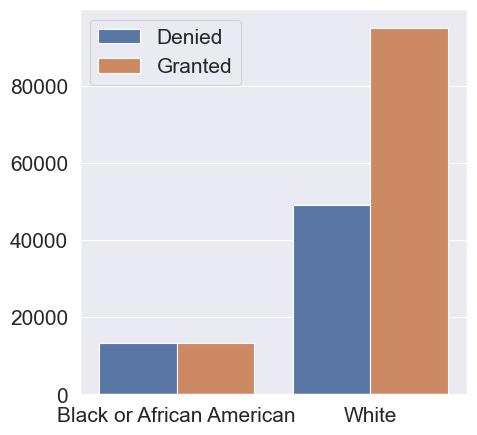
\includegraphics[width=\linewidth, valign=t]{images/loan_grants_by_protected_attributes/initial.png}
        \end{subfigure}
    \end{minipage}%
    \begin{minipage}[b]{0.5\textwidth}
        \centering
        \begin{subfigure}[t]{0.06\textwidth}
            \textbf{b)}
        \end{subfigure}
        \begin{subfigure}[t]{0.9\textwidth}
            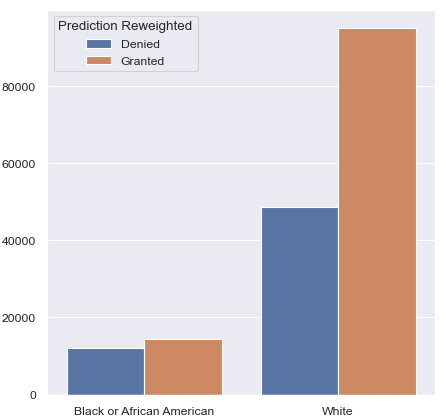
\includegraphics[width=\linewidth, valign=t]{images/loan_grants_by_protected_attributes/reweighted.png}
        \end{subfigure}
    \end{minipage}%
    \hfill\allowbreak%
    \begin{minipage}[b]{0.5\textwidth}
        \centering
        \begin{subfigure}[t]{0.06\textwidth}
            \textbf{c)}
        \end{subfigure}
        \begin{subfigure}[t]{0.9\textwidth}
            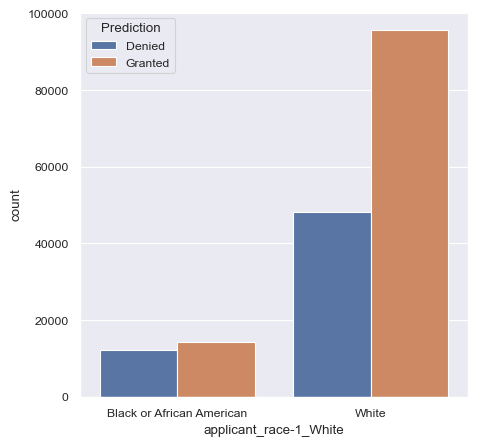
\includegraphics[width=\linewidth, valign=t]{images/loan_grants_by_protected_attributes/correlation_removed.png}
        \end{subfigure}
    \end{minipage}%
    \begin{minipage}[b]{0.5\textwidth}
        \centering
        \begin{subfigure}[t]{0.06\textwidth}
            \textbf{d)}
        \end{subfigure}
        \begin{subfigure}[t]{0.9\textwidth}
            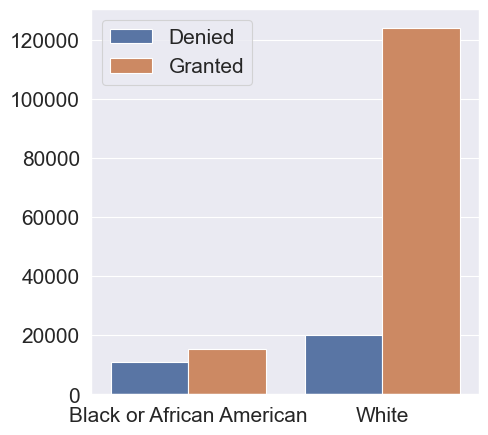
\includegraphics[width=\linewidth, valign=t]{images/loan_grants_by_protected_attributes/calibrated_eqodds.png}
        \end{subfigure}
    \end{minipage}%
    \caption[Differences in Positive Predictions per Model]{\textbf{Differences in Positive Predictions per Model} - Only the \textit{Calibrated Equalized Odds} model \textbf{d)}, which exhibits a higher amount of overall predicted grants, changed the ratio of granted mortgages among the races significantly compared to the benchmark model \textbf{a)}.
    The \textit{reweighted} model \textbf{b)} and the \textit{correlation removal} model \textbf{c)} did not significantly change the ratio.}
    \label{fig:Bar_Grant_per_Race}

\end{figure}

\textbf{Figure \ref{fig:Fairness_Adjustments_Results_Line}} shows the results of the fairness adjustments in terms of the \textit{disparities} of the model. The disparities were calculated for the \textit{true positive rate}, the \textit{false positive rate}, the \textit{true negative rate}, and the \textit{false negative rate}. 
The disparities were calculated for the \textit{White} and \textit{Black or African American} applicants. As they are relative terms, only the relation of the disparities to the other group is shown.
The disparities were comparably low for the \textit{true positive rate}, while all the other disparities show at least one outlier. The \textit{reweighed} model was the only one that produces satisfactory results in terms of fairness as measured by disparities across all four KPIs, with the benchmark model coming in second.

\begin{figure}[!htbp]
    \centering
    \includegraphics[width=0.85\textwidth]{images/CHXX_Update_Results_Line.png}
%    \caption{Fairness Adjustments Results}
%    \medskip
%    \small
%    The results of the fairness adjustments in terms of the disparities of the model. The disparities were calculated for the \textit{true positive rate}, the \textit{false positive rate}, the \textit{true negative rate}, and the \textit{false negative rate}. They were calculated for the \textit{White} and \textit{Black or African American applicants}. Values closer to 1 are better, the gray area represents a good level of fairness.
    \caption[Fairness Adjustments Results]{\textbf{Fairness Adjustments Results} - The results of the fairness adjustments in terms of the disparities of the model. The disparities were calculated for the \textit{true positive rate}, the \textit{false positive rate}, the \textit{true negative rate}, and the \textit{false negative rate}. 
    They were calculated for the \textit{White} and \textit{Black or African American applicants}. Values closer to 1 are better, the gray area represents a good level of fairness.}
    \label{fig:Fairness_Adjustments_Results_Line}
\end{figure}

Adding up all fairness metrics for all iterations (see \textbf{table \ref{tab:metrics_2_iterations_summary}}) resulted in a mixed picture.
While the \textit{reweighing} algorithm managed to improve the fairness of the outcomes in terms of disparities (as can also be inferred from \textbf{figure \ref{fig:Fairness_Adjustments_Results_Line}}), the predictive power of the model for subgroups did not show a single optimal model.

\begin{table}[!htbp]
    \centering
    \begin{tabular}{l *{4}{>{$}c<{$}}}
    \toprule
    & \textbf{Initial Model} & \textbf{Reweighing} & \textbf{Calibrated Equalized Odds} & \textbf{Correlation Removal} \\
    \midrule
    \textbf{Accuracy White} & 0.91 & 0.91 & 0.72 & \textbf{0.91} \\
    \textbf{Precision White} & \textbf{0.89} & 0.89 & 0.68 & 0.89 \\
    \textbf{Recall White} & 0.97 & 0.97 & \textbf{0.98} & 0.98 \\
    \textbf{F1 Score White} & 0.93 & 0.93 & 0.81 & \textbf{0.93} \\
    \textbf{AUC White} & \textbf{0.94} & 0.94 & \text{NA} & \text{NA} \\
    \midrule
    \textbf{Accuracy Black} & 0.88 & 0.88 & 0.81 & \textbf{0.89} \\
    \textbf{Precision Black} & 0.82 & 0.81 & 0.73 & \textbf{0.84} \\
    \textbf{Recall Black} & 0.96 & \textbf{0.97} & 0.93 & 0.93 \\
    \textbf{F1 Score Black} & 0.88 & \textbf{0.88} & 0.82 & 0.88 \\
    \textbf{AUC Black} & \textbf{0.95} & 0.95 & \text{NA} & \text{NA} \\
    \midrule
    \textbf{tpr\_disparity} & 0.99 & \textbf{0.99} & 0.95 & 0.96 \\
    \textbf{fpr\_disparity} & 0.96 & \textbf{1.00} & 0.43 & 0.80 \\
    \textbf{tnr\_disparity} & 1.01 & \textbf{1.00} & 2.23 & 1.05 \\
    \textbf{fnr\_disparity} & 1.42 & \textbf{1.20} & 3.25 & 2.67 \\
    \bottomrule
    \end{tabular}
%    \caption{Metrics \#2: Fairness Adjustments Summary}
%    \small
%    Results of \textit{metrics \#2} for all applied algorithms. The values are rounded, the highest scores (respectively those closest to 1 for the disparity calculations) are marked \textbf{bold}.
    \medskip
    \caption[Metrics \#2: Fairness Adjustments Summary]{\textbf{Metrics \#2: Fairness Adjustments Summary} - Results of \textit{metrics \#2} for all applied algorithms. The values are rounded, the highest scores (respectively those closest to 1 for the disparity calculations) are marked \textbf{bold}.}
    \label{tab:metrics_2_iterations_summary}
\end{table}